\documentclass[a4paper]{article}

\usepackage[english]{babel}
\usepackage[bitstream-charter]{mathdesign}
\usepackage[T1]{fontenc}
\usepackage{graphicx}


\begin{document}
\selectlanguage{english}

\title{Comparative Programming Languages\\
Assignment $^{\#}$2: Domain Specific Language}
\author{Glenn Croes \and Philippe De Croock \and Thomas Winant}
\date{11 January, 2012}

\maketitle

\section{Domain description}
\label{sec:domain-description}

% An elaboration on elements of the domain that were missing or needed to be improved, plus justification for any choices made.


\section{Domain analysis}
\label{sec:domain-analysis}
% A brief breakdown of the elements in your domain and how they relate to each other. This could be a formal meta-model, but could also be textual description.

\begin{figure}[ht!]
  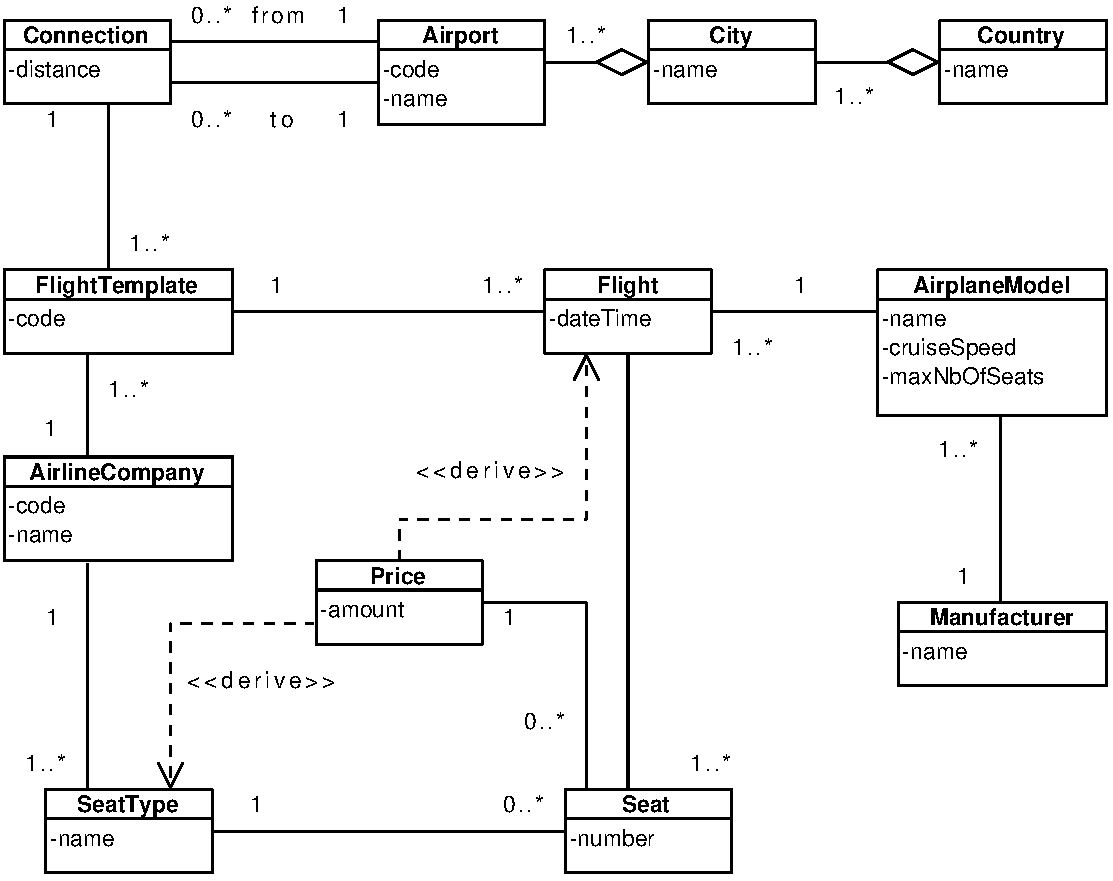
\includegraphics[width=1.0\textwidth]{../analysis/domainModel.pdf}
  \caption{Domain Model}\label{fig:domain-model}
\end{figure}


\section{Design description}
\label{sec:design-description}


\begin{figure}[ht!]
  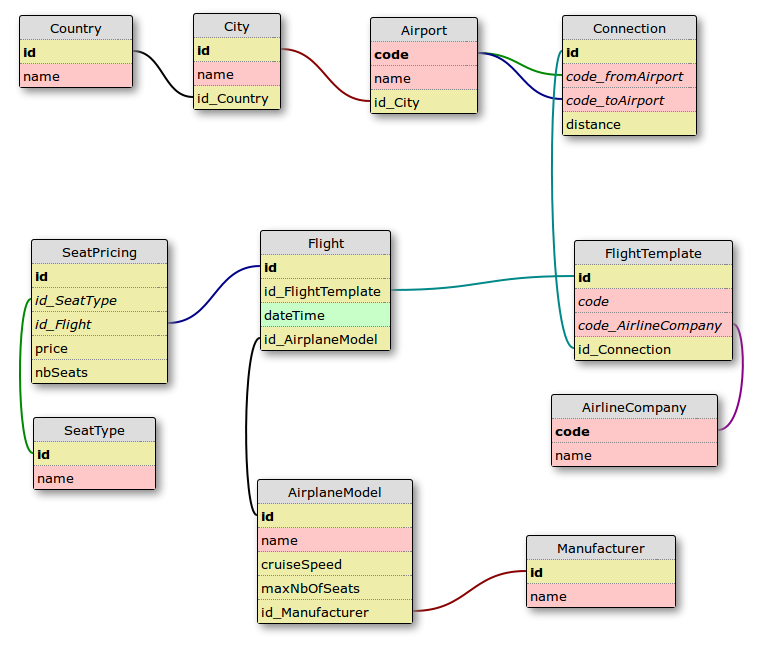
\includegraphics[width=1.0\textwidth]{../analysis/dbtables-diagram.png}
  \caption{Database Tables}\label{fig:database-tables}
\end{figure}


% A description of the semantic model underlying the DSL, along with a description of the constructs of your DSL.

\section{Implementation overview}
\label{sec:implementation-overview}

% A general overview of the implementation approach, including a description of the API upon which it is based and any tricky implementation techniques employed. Some justification of the chosen implementation language needs also to be provided.

\section{DSL Implementation}
\label{sec:dsl-implementation}

% The code implementing your DSL and any libraries on which it is based.

\section{Example DSL program(s)}
\label{sec:example-dsl-programs}

% Some example DSL programs to illustrate how your DSL is to be used.

\section{Guide}
\label{sec:guide}

% to use A short description of how to compile and run your DSL and a guide to the structure of the submitted files.



\end{document}


%%% Local Variables:
%%% mode: latex
%%% TeX-master: t
%%% End:
